\documentclass[]{revtex4-1}

\usepackage[fleqn]{amsmath}
\usepackage{amssymb,amsthm}
\usepackage[dvips]{graphicx}
\usepackage{color}
\usepackage{tabularx}

\newcommand{\recheck}[1]{{\color{red} #1}}
\newcommand{\redc}[1]{{\color{red} #1}}
\newcommand{\bluec}[1]{{\color{blue} #1}}
\newcommand{\greenc}[1]{{\color{green} #1}}
\newcommand{\vect}[1]{\textbf{\textit{#1}}}
\newcommand{\dd}[1]{\textsf{#1}}
\newcommand{\fwd}[0]{\textrm{fwd}}
\newcommand{\bwd}[0]{\textrm{bwd}}
\newcommand{\period}[0]{T_{\textrm{P}}}

\begin{document}

\section*{The scientific issues from referee 1}

\emph{On a principle level I am not sure that the relevant scientific
  question is really the non-equilibrium response since the response
  to the external field -- as the authors note -- is indeed quite
  fast. In fact, most of the discussion in the paper is focused on
  what I think could have been extracted just as well from
  conventional equilibrium simulations (conformational shifts,
  kinetics).}\\

The non-equilibrium responses in the paper are discussed in two
different senses: 1, the perturbation to the system is
time-independent.
The relaxation of the system to the new equilibrium
defined by the constant perturbation is non-equilibrium.
% However,
% after the new equilibrium is established, there is no non-equilibrium
% process in the system.
The first example of the manuscript is in this sense.  2, the
perturbation is time-dependent.  The second example in the manuscript
is in this sense.  The first sense is only a special case of the
sencond sense.  In the first sense, the system can be studied by
equilibrium methods such as the Markov state model (MSM). However, the
equilibrium methods are NOT applicable in the second sense.  The
present paper develops a non-equilibrium molecular dynamics simulation
method that is more general in the sense that it is applicable to the
aformentioned two senses. Therefore, the proposed method cannot be replaced
by the equilibrium methods such as MSM.

Another commenly used equilibrium method that is able to study the non-equilibrium
responses is the linear responses thoery (Green-Kubo relation).
We also use it to test the
conformational shift of alanine dipeptide under the electric field
(EF). The response function, take the time-dependent probability of
left-handed $\alpha$-helix (Conformation $C$ in the old manuscript. The notation has been changed to $\alpha_L$ in the updated manuscript.) for example, is defined as
\begin{align}\label{eqn:tmp1}
  P_C(t) = \langle\chi_{_C}(t)\rangle = \langle \chi_{_C} \rangle_0 -
  \beta \int_0^t ds\; M_e(t - s)\langle j(0)\cdot \chi_{_C}(t) \rangle_0
\end{align}
where $\chi_{_C}$ is the characteristic function of set $C$ that takes
the value of 1 for $(\phi,\psi)\in C$, and takes value 0
otherwise. $M_e(t)$ is the magnitude of the EF. In the case of
constant EF, $M_e(t) = t/t_{warm}$ for $0\leq t<t_{warm}$, and
$M_e(t) = 1$ for $t\geq t_{warm}$.
$j$ is the dissipative flux that is defined by
\begin{align}
  j = - \sum_{i=1}^N E_\infty q_i v_{i,x},
\end{align}
where $q_i$ is the partial charge of the $i$th atom, and $v_{i,x}$ is
the $x$ component of the velocity of the $i$th atom.  The notation
$\langle\cdot\rangle_0$ denotes the equilibrium ensemble average.
Eq.~\eqref{eqn:tmp1} can be found in the text books of statistical
mechanics (e.g.~M.~Tuckerman \emph{Statistical Mechanics: Theory and
  Molecular Simulation}, pp.~499).  We plot the correlation function
$\langle j(0)\cdot \chi_{_C}(t) \rangle_0$ against corrlation time $t$
in Fig.~\ref{fig:tmp1} of this reply. The value of the function is estimated from
two independent equilibrium simulation, and the trajactory of each is
of 1~$\mu$s. Please note that the total length of the equilibrium
trajactories is the same as the non-equilibrium simulation (2000
trajactories, each 1000~ps long).
% With the knowledge of
% non-equilibrium simulation, the correlation function is expected to
% vanish at roughly 500~ps, however, it does not vanish even at
% 1000~ps. This is not surprising, because
We find that the statistical error is even larger than the value of
corrlation function.  Therefore, the
overwhelming statistical uncertainty does not allow us to use it 
in Eq.~\eqref{eqn:tmp1} to calculate the
non-equilibrium averages. 
% , and we actually do not know when the
% corrlation function vanish .
Since the total computational effort of
the equilibrium simulation is the same as the non-equilibrium
simulation, we conclude that non-equilibrium simulatoin is more
precise than the conventional equilibrium approach (linear response) at the same computational cost.
A similar
observation has already been reported by Ciccotti and Jacucci, PRL
1975.
\\
% Another limit of the linear response theory is that it can only be
% used to calculate the non-equilibrium properties when the
% non-equilibrium purturbation to the system is small, and it is also
% impossible to tell \emph{a priori} if the purturbation is small enough
% that the response theory is valid. This issue also does not exist in
% our non-equilibrium simulation method.


\begin{figure}
  \centering
  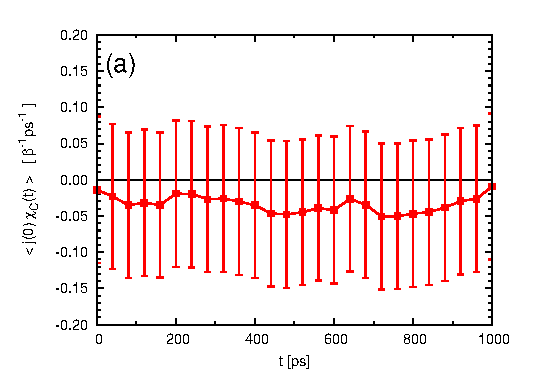
\includegraphics{figs/fig-corr-meta.eps}
  \caption{The corrlation function $\langle j(0)\cdot \chi_{_C}(t)
    \rangle_0$ against time $t$. The error bars in the figure denote
    the statistical uncertainty at 95\% confidence level. }
  \label{fig:tmp1}
\end{figure}


\emph{
In the alanine dipeptide system studied here, I am not sure that the
initial simulation is in fact fully converged and -- if the question is
how conformational preferences evolve in response to an external field
-- whether the short branch simulations are long enough to establish
convergent sampling. More specifically, I think that the lack of
sampling of the left-handed helix in the absence of an electric field
is a result of insufficient sampling to cross the kinetic barrier from
beta to alphaL conformations (alanine dipeptide with CHARMM27 has been
extensively characterized and I suggest a comparison with relevant
papers from MacKerell et al.). If such relevant conformations are
missing from the initial snapshots and the branch simulations are
short I am concerned that the resulting initial bias affects the
non-equilibrium results.
}\\

We have done an equilibrium simulation of 1~$\mu$s.  On the
trajactory, molecular conformations are recored every 500~ps,
therefore, in total 2000 equilibrium conformations are recoreded.  The
equilibrium probabilities of the conformations $A_1$, $A_2$, $B_1$,
$B_2$ and $C$ are 0.426 ($\pm 0.029$), 0.076 ($\pm 0.010$), 0.265
($\pm 0.013$), 0.182 ($\pm 0.019$) and 0.051 ($\pm 0.021$),
respectively.  We have run two addtional equilibrium simulations of
1~$\mu$s, and the probabilities of conformations are consistent with
the values listed above, which means that our new equilibrium
simulation is fully converged.  Comparing with our previous
equilibrium simulation (only 0.1~$\mu$s long),
% in which the
% probability of left-handed $\alpha$-helix is only 0.008,
the precision
of initial configuration sampling is substantially improved. All
simulations in the manuscript are reperformed according to the new set
of initial conformations, however, the strand of all time-dependent
observables are the same as the old simulation, and no change to the
conclusions is made.
% The difference between the new and the old
% results is no more than 0.05, which is basically within the
% statistical uncertainty (given in the new manuscript).

We also test the convergence of simulation result with respect to the
number of branching trajactories.  The time-dependent probabilities of
each conformation calculated from one branching trajactory is compared
with four braching trajactories (each of them is simulated with
different random seed for Langevin thermostat) in
Fig.~\ref{fig:tmp2} of this reply. The results are consistent, which means that the
sampling of the non-equilibrium trajactories is fully converged. In
summary, since the our non-equilibrium simulation includes the
sampling of both initial configurations and non-equilibrium
trajactories, the convergence of both aspects implies the convergence
of our simulation results.

The question on whether our non-equilibrium braching trajactories are
long enough so that the results are fully converged is a very subtle
question. There may exists an intrisic time-scale of 1 microsecond
long, so we cannot discover it by braching trajactories of only a few
nanoseconds.  What we can do by the proposed non-equilibrium simulation
method is to study time-dependent behaviours that are no longer than
the simulation time. We have modified the manuscript according to
make this point clear. A similar difficulty actualy exists for all equilibrium
simulations: how do we know whether an equilibrium simulation is fully converged,
especially when some rare events cannot be observed during the limited simualtion time.
\\
% We want to stress that the target of the non-equilibrium simulation is
% to test how the populations of conformations evolve under the external
% electric field

\begin{figure}
  \centering
  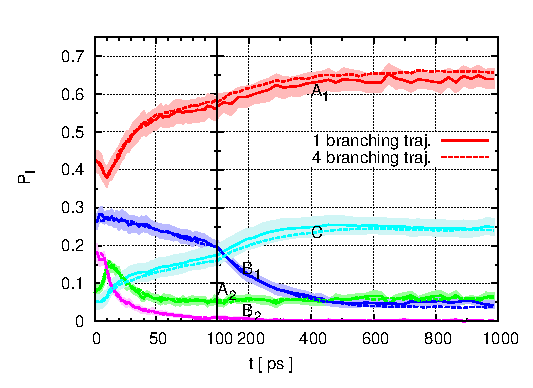
\includegraphics{figs/fig-meta-more.eps}
  \caption{A comparison between the simulation with one branching
    trajectory per every initial conformation and four branching
    trajectories  for the
    constant EF case. Each of the four
    branching trajectories is simulated with a different random seed for
    Langevin thermostat.
    The shadow region presented with each line of the one-branching-trajectory case
    denotes its statistical uncertainty at 95\% confidence level.  }
  \label{fig:tmp2}
\end{figure}

\emph{ It looks as if the CMAP correction was used with the CHARMM
  force field but no information is given in the methods section.}\\

Yes, the CMAP correction is used. We mention it in the
section III.A. of the updated manuscript.
\\

\emph{
I am curious how the choice of Rex for the thermostat would affect the
results.
}\\

We compared the simulation results of two different $R_{ex}$ values:
1.0~nm and 1.5~nm in Fig.~7 (pp.15) of the manuscript. The
$R_{ex}=1.0$~nm case was simulated in periodic cubic simulation box
of length $L=2.7$~nm and 4.0~nm.  The $R_{ex}=1.5$~nm case was
simulated in cubic box of length $L=4.0$~nm. Fig.~7 of the
manuscript demonstrates that all of the results are consistent. That
means $R_{ex}=1.0$~nm is already large enough, and a larger $R_{ex}$
would not change the results.\\

\emph{ I wonder about the motivation of using electric fields with
  periods of 10, 40, and 200ps. How do such fields relate to the
  practical question of electromagnetic radiation exposure?  }\\

The periods 10, 40~ps are roughly the same as the first two shortest
time scales of probability fluxes observed in the constant EF case,
see Table~I of the manuscript. We tried to simulation with period of
500~ps, which is the same as the longest timescales of the constant EF
case, however, the required simulation time is so long that exceed our
computational capability. Therefore, we made a compromise that only
the period of 200~ps is studied. The typical frequency of the microwave
irradiation is 2450~MHz, which corresponds to period of 400~ps. It is
the same order of magnitude as the $T_P=200$~ps studied by us.
\\

\emph{ The analysis of ``probability fluxes'' seems to be nothing else
  than a kinetic analysis. Maybe some comments on how these are
  related would be helpful.  }\\

Yes, the definition of the probability fluxes is similar to the
kinetic rate (we use joint probabilities in (6) rather than
conditional probabilities). However, we want to stress that, in genarl,
the probability fluxes calculated in the manuscript should not be
interpreted as a kinetic rate, and one cannot replace the
non-equilibrium molecular dynamics by a kinetic analysis. The main
reason is two folds:
Firstly, for a non-equilibrium system, the probability fluxes are
time-dependent, therefore, the lag-time $\Delta t$ in the definition (Eq.~(6))
should be small comparing with the typical time-scale of conformation change.
Secondly, for a small lag time $\Delta t$ (1~ps in the manuscript), the conformational
dynamics of biomolecules is generally not
Markovian (see e.g.~C.~Sch\"utte et.~al.~JCP 2011 and J.-H.~Prinz et.~al.~JCP 2011).
Since the basic assumption -- Markovianity -- of the kinetic analysis
may not be satisfied, a direct
application of the kinetic analysis in the non-equilibrium cases is questionable. Although one may
gain usefuly information from the kinetic analysis, the reliability
and the effectiveness of this approach should be carefully checked case
by case.  Since the main goal of our research is to propose a
non-equilibrium molecular dynamics simulation method, the numerical
results are not compared with a kinetic analysis.

A comment on this direction has been added to the end of section III.B.
\\

\emph{Finally, given the apparent convergence issues with alanine
  dipeptide I have difficulties seeing how this method could be
  applied in a reasonable manner to more complex systems. Maybe some
  comments to that extent would be helpful.  }\\


Please see the reply to the seocond question concerning the convergence
of our simulation results. We believe that the better initial
state sampling and the new convergence check with respect to the
number of branching trajectories will strengthen the reliablity
of our method.
% manuscript and



% We have added a section in the appendix in the manuscript discussing
% the convergence and reliablity of our method. Please also see the
% answer to the 2nd question.



\section*{The scientific issues from referee 2}

\emph{
It would be useful if the authors would briefly comment on the
relationship between time-varying electric fields and terahertz
spectroscopy. Experimental work in this frequency range may be related
directly to the results reported here. See work by Plusquellic et al
(ChemPhysChem 2007), Havenith et al. (Faraday 2009) and others.
}\\

The frequency investigated in our manuscript is from 5~GHz to 100~GHz,
the largest of which is still one order of magnitude smaller than the
terahertz spectroscopy. Therefore, we find our simulation results
cannot be directly compared with the terahertz experiments.\\

\emph{ The procedure for controlling the temperature under neq
  conditions is reminiscent of the ``stochastic boundary conditions''
  introduced by Brooks and Karplus (JCP 1983). Can the authors provide
  a more formal description of their procedure and touch on
  similarities/dissimilarities with the Brooks/Karplus approach?  }\\

Yes, a comment and comparison on this direction has been added to the
manuscript.\\

\emph{ In the methods sections the treatment of H-involving bonds is
  not explained (SHAKE, RATTLE, ??). Also, a reference for the TIP3P
  model should be given. What cutoffs are required for an "energy
  conserving PME" simulation and how were the vdw interactions
  handled?  }\\

The asked details has been added to the manuscript.\\

\emph{
It is suggested to adapt the labeling of the conformational substates
of alanine dipeptide to that used in the literature ($C_7^{eq}$, $\alpha_L$,
$C_7^{ax}$, etc.) - see e.g. Caflisch et al., JCP 1999.
}\\

We have changed the labelling of conformations.\\

\emph{
The sentence ``..how the behaviour of the electric dipole moment of the
molecule is influenced..'' reads somewhat strange. Obviously, each of
the metastable states has its own dipole moment and this is reported
later on p. 12. However, there is no reason why the EF should
\emph{influence} the dipole moment as the simulations employ a force field
with fixed charges. It would probably be helpful to clarify that the
EF leads to ``conformational selection'' through alignment of the
molecular dipole along the EF.
}\\

We have made corresponding changes to the manuscript.\\

\emph{ It would be interesting to relate the probability fluxes from
  Fig 11 to the work by Rao et al. (PNAS 2007) and the Caflisch JCP
  1999 article. It should be possible to relate the probability fluxes
  to free energy differences.}\\

This is indeed a very interesting point. Although the Fig.11 is
plotted for the non-equilibrium oscillatory EF case, the
confromational transition pathways are qulitatively comparable to the
previous works on the transition pathways studied in equilibrium.
Both the connectivity of conformations and the relatively strength of
the transitions are similar. A short comment has been added to the
manuscript.

The transition fluxes can be used to calculate the free energy only in
the equilibrium case. In the non-equilibrium cased, especially the
oscillatory EF case, the conformational kinetics of the system is generally
not Markovian. Therefore, the standard kinetic analysis cannot be used
here.

\end{document}
